\section{Experimental Results}
Unfortunately we were not able to utilize the DAS-4 system (due to an incompatible Java version), however we tested the game when running on two different laptops over a local area network (LAN). These tests were after the initial deadline and therefore the testing part of the game had already been done. Therefore we decided to spend this chapter on how we wish we could have performed the experiments in the first place if these implementation problems hadn't delayed us this much. However we were able to collect some primitive data from some local experiments. These results will be discussed here as well.

\subsection{Setup}
The code of the DAS game, which was used for these experiments, is made publicly available under the BSD new license and is available on: \url{https://github.com/pbrand/DCS-Dragon-Arena-System}. 
The license can be reviewed at: \url{https://github.com/pbrand/DCS-Dragon-Arena-System/blob/development/Game/LICENSE}
For this experiment, the DAS-4 should be initialized with 5 compute-nodes. 
One compute node should host the main server which initializes the battlefield. 
Another compute node should initialize the backup for the main server (the backup server). 
Another 2 nodes should be used as the helper servers which connect to the main server. 
Finally the last node can be used to instantiate 3 clients which connect to the randomly distributed helper server nodes.

\subsection{Consistency Experiments}
The purpose of causal consistency is to make sure that events that are causally related are actually ordered. 
To measure this, it is necessary to assign a timestamp upon message creation. 
Additionally, each message is provided with its own unique identifier. 
Every message which is received should be stored in a list and assigned a timestamp which represents the time of arrival.
Whenever a new message is received, its timestamps should be checked with the other timestamps of messages in the list in order to check causality. If the newly received message was sent before a message which had already been received earlier, and these messages are causally related, then the causality constraint is certainly not met.
In this project, a causal relationship is defined by: a certain unit \emph{A} performs an action which has an effect on the state of a certain unit \emph{B}, for instance if a player \emph{A} attacks a dragon \emph{B}.

It is also important to measure how consistent the backup of the battlefield is with the battlefield on the main server.
This can be measured by taking a snapshot of the battlefield on the main server at a random time after which the main server is forcefully shut down. 
At this moment, the taken snapshot can be compared with the latest backup of the battlefield at the backup server. 
The difference in location of the units are an indicator of the consistency between the backup and the main server. The difference in health points of the units can be a measure as well. The combination of these two measures will give a rough indication of the divergence of the backup compared to the main server. 
A more concrete measurement can be obtained by backing up the previously mentioned list of messages and checking the differences between both battlefields. The amount of missing messages in the backup is the exact number of events that were lost during the recovery, hence a clear indication of the inconsistency. 
This experiment should be performed several times in order to guarantee an unbiased result, as the random time of the snapshot will probably sample at different times after the creation of the latest backup at the backup server. 

\subsection{Scalability and Performance Experiments}
In order to test scalability it is important how scalable the helper servers are and how scalable the main server is. 
First, to test the scalability of the helper servers, it is important to have just one variable in this test environment. 
The variable for the scalability of the helper server test lies in the amount of connected clients. 
Therefore we have one fixed main server and one helper server.
The number of connected clients are increased per test run. 
During the tests, the system of the helper server is monitored.
Just like in the previous section, the messages and their timestamp are also recorded.
For each test run, the average response time can be computed.
Then, these response times can be compared which each other in order to check if an increase in clients has an impact on the response time of the server.
If the response time dramatically increases, it is clear that the system is limited to the number of clients it can scale to. 
This is also an indicator for the performance of the system.
The memory and CPU usage should also be recorded  and compared with each other for each test run in order to find the performance bottleneck. 
The only constraint is, that the same hardware is used during every test run.

It is also important to test how scalable the main server is. 
As already stated, there is only one main server active, but the number of helper servers may be increased.
This test will measure  the number of helper servers the main server can handle.
The number of clients per helper server will be kept consistent for each test in this experiment, only the number of helper servers will be increased for each following test run.
The same properties as in the scalability of the helper servers will be measured, but now for the main server.
Instead of measuring the response time of messages between helper and client, the response time between helper and main server is measured.
The CPU and memory usage are also recorded in order to find the performance bottleneck.


\subsection{Fault-Tolerance Experiments}
For fault tolerance the system also needs to be tested for both the helpers and the main server.
To test the tolerance of the system when helpers crash, tests are run with multiple helper servers which are killed at random to simulate crashes.
It is then possible to measure the number of messages which were tried to be sent from the server and the number of messages which were actually sent to a helper server after one was randomly killed.
These tests need to be run multiple times and the different outcomes should be compared in order to get a view of the number of failed sent messages.
If this value is low, it is probably safe to conclude that the helper server's fault-tolerance is acceptable.

The same experiment should be done for measuring the tolerance of the main server.
Instead of killing a helper, the main server should be killed, and then the backup server should take over the responsibilities of the main server.
During this test, the number of missing messages (events) should be measured by taking the difference between the number of messages on the backup server and the main server, just like it is explained in the section about the scalability.
Also, the number of failures after the backup server is promoted to main should be taken into account.
The less failures after the restore, the better the recovery mechanism is.

\subsection{What actually happened}
% Setup
During the implementation of the game, the game was mainly tested on the local machines.
To simulate the distribution of the system locally, different RMI registries were used for the main classes which are supposed to run on different nodes.
By doing so, the running classes need to call a different (local) server in order to make an RMI call.

% Consistency
As stated in the previous chapter, the helper server does not maintain a state of the game, but sends messages to retrieve the required information in order to perform the computation. 
A number of tests were run to measure the traffic for messages sent, received and failed to sent by the helper server.
These results are from tests in which the system is spawning the players by reading a file from the Game Trace Archive.
No helper nodes were killed.
It is still notable that there are some messages failing to be sent. 
However the number of messages which failed is really small (therefore not visible in results chart).
The results can be seen in figure \ref{helper_pie}.

%What is also observed, is that the failures in the helper servers is much lower than the failure in the main server.
%This is probably because the main server eventually receives many more requests than each helper server.

\begin{figure}[ht]
\centering
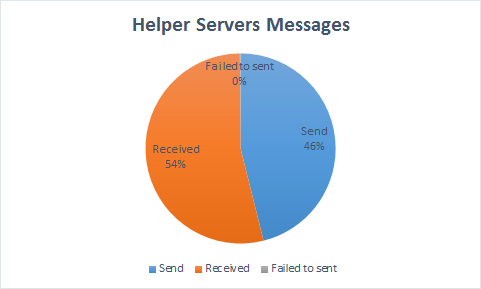
\includegraphics[scale=0.8]{images/helper_pie.png}
\caption{Helper Server Messages}
\label{helper_pie}
\end{figure}

The same data was also collected for the main server when running these tests.
The results are shown in figure \ref{master_pie}.
In this figure it is notable that there are about 1\% of messages failing.
This may seem small in percentage, but it may definitely not be ignored in terms of number of messages.
The reason for more failing messages at the main server is because it needs to handle more messages than the helper server, it receives in total more messages than the helpers combined.
What is interesting to see, in contrast to the helper servers, the number of messages sent is almost twice as the number of messages received.
This is due to the fact that the main server sends less messages back to clients than the helpers do.
For instance: when clients perform a move they do not get a message back of an acknowledgement of the move.

\begin{figure}[ht]
\centering
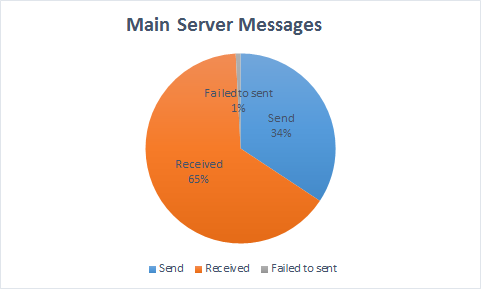
\includegraphics[scale=0.8]{images/master_pie.png}
\caption{Master Server Messages}
\label{master_pie}
\end{figure}

For scalability tests we did not collect hard evidence. 
However, there we did run some tests in which random helper servers were killed after which the clients reconnected to other helper servers.
The clients were also able to continue playing the game.
In the charts from figures \ref{helper_hist} and \ref{master_hist}, the number of messages sent, received and failed can be seen per test run for helper and master server.
For each following test, the number of clients were increased. 
Obvious observation: the more clients, the more messages there are sent and received.

\begin{figure}[ht]
\centering
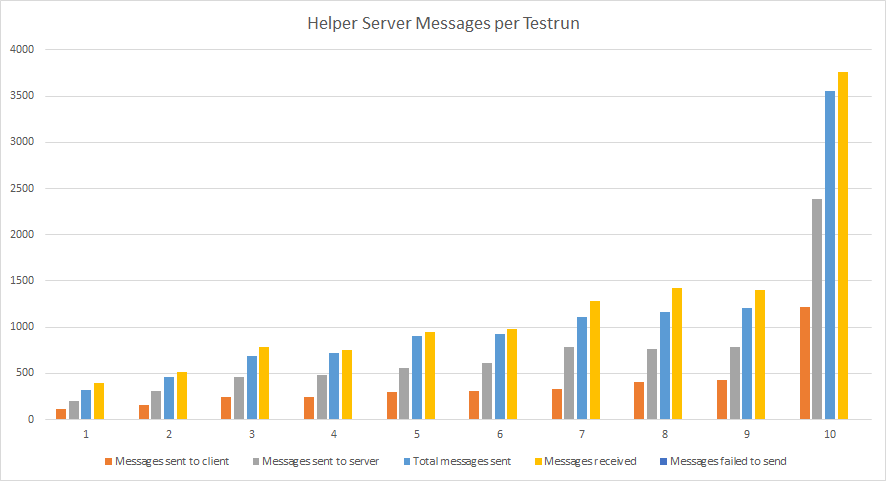
\includegraphics[scale=0.8]{images/helper_hist.png}
\caption{Helper Server Tests}
\label{helper_hist}
\end{figure}

\begin{figure}[ht]
\centering
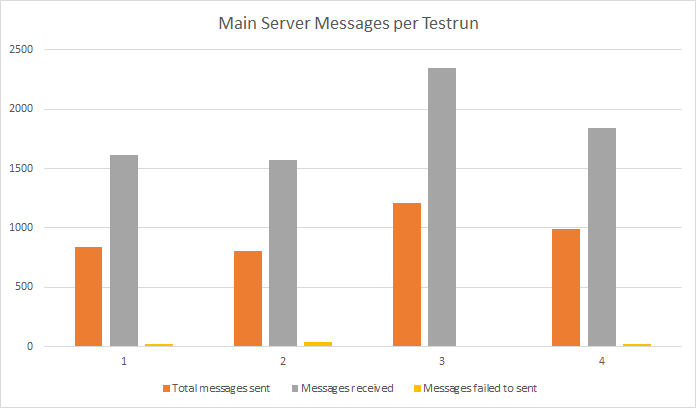
\includegraphics[scale=0.8]{images/master_hist.png}
\caption{Master Server Tests}
\label{master_hist}
\end{figure}

Another thing which can be noted from the metrics result (figure \ref{client_helper}), is that the nodes are quite balanced.
Even though the helper servers are chosen at random it still shows that every helper node has a fair amount of clients.
During the tests there was no case in which almost all clients were connected to one server node and every other helper was doing almost nothing.
Because these nodes are quite balanced, clients can reconnect faster to other helper nodes, simply because the number of helper nodes which need to reconnect is not large.

\begin{figure}[!ht]
\centering
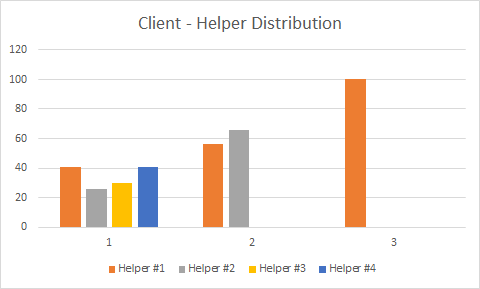
\includegraphics[scale=0.8]{images/client_helper.png}
\caption{Clients and Helpers Distribution}
\label{client_helper}
\end{figure}

In figure \ref{client_helper}, the first test was run with four helpers, the second with two clients and the third with only one.
Obviously all clients were forced to connect to the only available helper server.

In the end we also tested the game on two laptops that were connected through a LAN. Although the game ran, some issues came up which were mainly related to updating the movement of the players. We think this is due to the great amount of messages that the main server needs to handle in a very short time period without any form of buffering.

